\chapter{Additional Information on Congestion-Free Simulation}\label{appendix:additional_info}

\begin{figure}[th]
	\centering
	\begin{subfigure}[b]{0.35\textwidth}
		\centering
		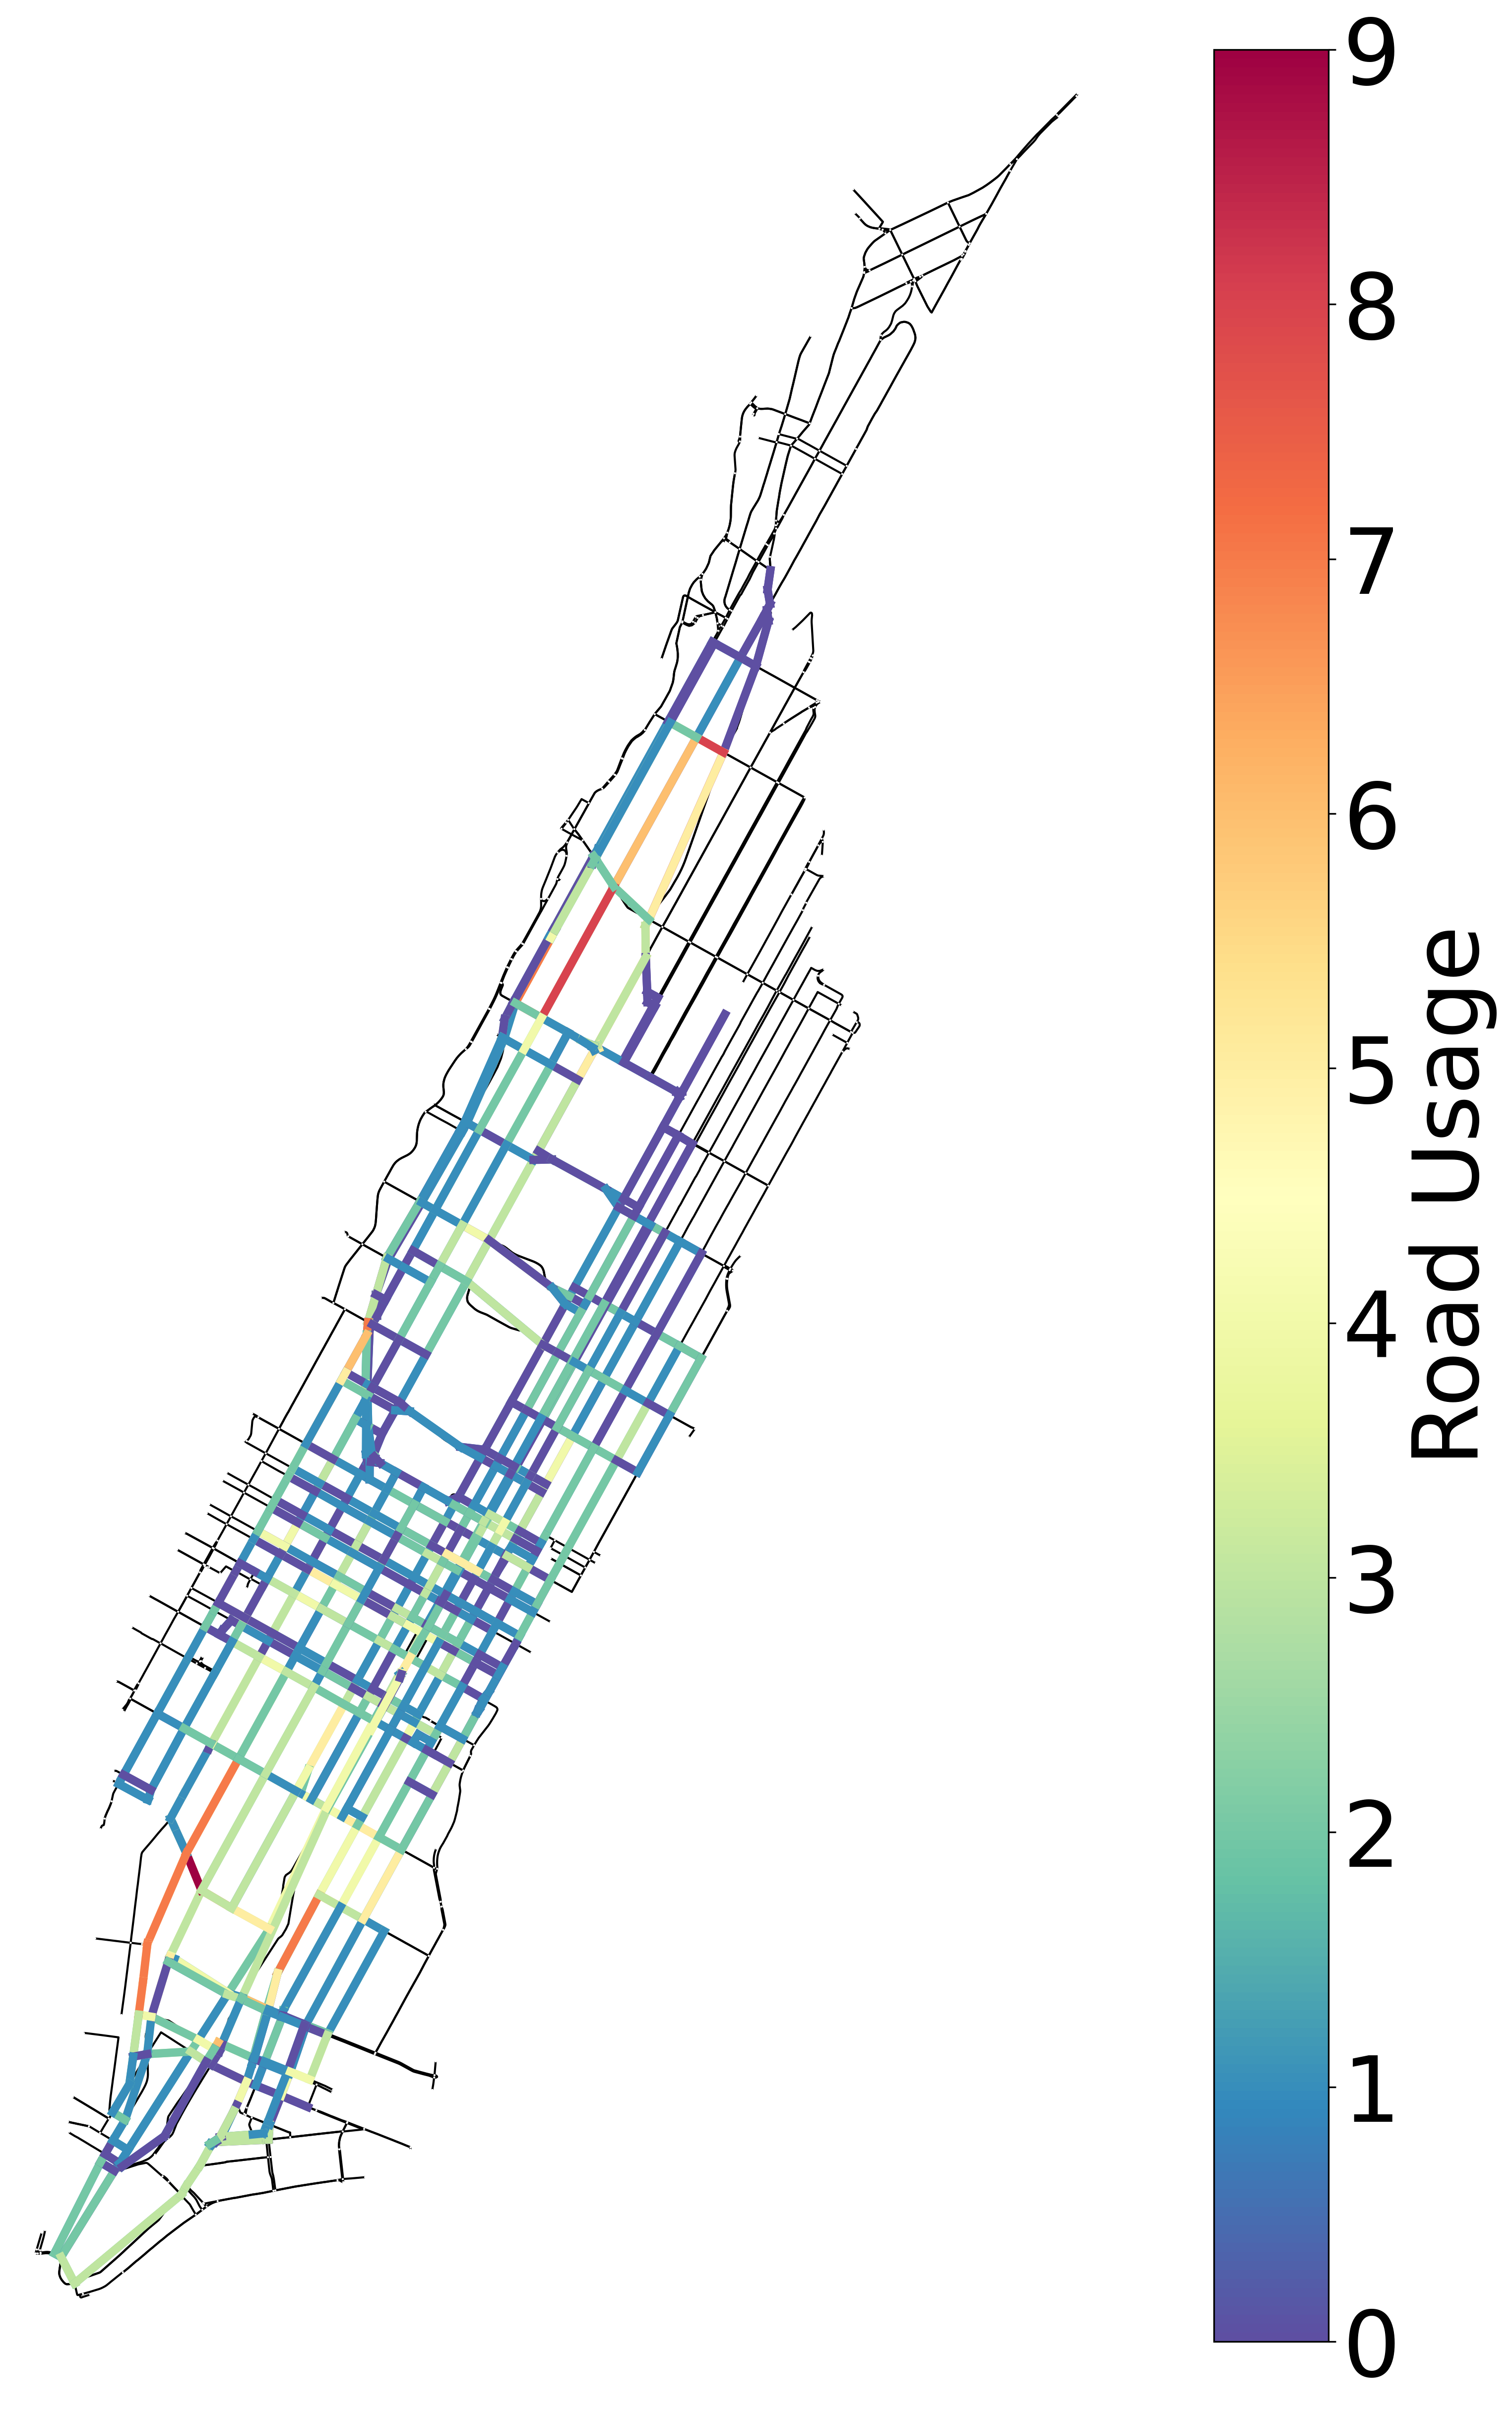
\includegraphics[width=\textwidth]{assets/img/appendix_a/nyc_road_usage_simu2.png}
		\caption{}
		\label{app:fig:nyc_road_usage_simu2}
	\end{subfigure}
	\begin{subfigure}[b]{0.4\textwidth}
		\centering
		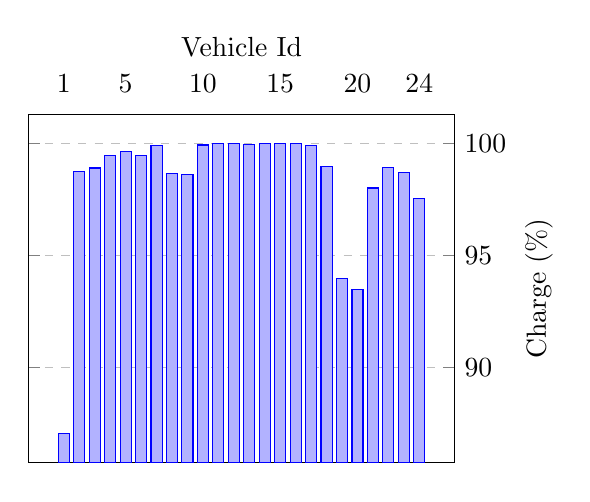
\begin{tikzpicture}
			\begin{axis}[
				ybar,
				xtick=data,
				xtick={1,5, 10,15,20,24},
				xlabel={Vehicle Id},
				ylabel={Charge (\%)},
				bar width=4pt,
				ymajorgrids=true,
				yticklabel pos=right,
				ylabel near ticks,
				grid style=dashed,
				xticklabel pos=right, xlabel near ticks,
				minor x tick num=9,
				xtick style={draw=none},
				width=7cm, 
				height=6cm
				]
				\addplot coordinates{
					(1,87.03273665754057)
					(2,98.75290642116234)
					(3,98.90571811652293)
					(4,99.47446699419078)
					(5,99.660626286003)
					(6,99.45728203892233)
					(7,99.91730734146344)
					(8,98.65314188361312)
					(9,98.59922346939065)
					(10,99.93223998867718)
					(11,100.0)
					(12,100.0)
					(13,99.94747727995325)
					(14,100.0)
					(15,100.0)
					(16,100.0)
					(17,99.92064289494235)
					(18,98.9835856552889)
					(19,93.97807766275497)
					(20,93.47662027131051)
					(21,98.01223510374761)
					(22,98.93486817125883)
					(23,98.71247932045945)
					(24,97.55665230827421)
				};			
			\end{axis}
		\end{tikzpicture}
		\caption{ }
		\label{app:fig:charge_vehicle_baseline_cong_simu2}
	\end{subfigure}
	\caption[Overview of System's Performance with Congestion Limits and Less Charging Time]{Overview of System's Performance without Congestion Limits and Less Charging Time.
		\subfigref{app:fig:nyc_road_usage_simu2} illustrates the utilization of the entire road network during the whole shift, while \subfigref{app:fig:charge_vehicle_baseline_cong_simu2} shows averaging charging percentage of the vehicles. 
	}
	\label{app:fig:nyc_analysis_congestions_simu2}
\end{figure}



\begin{figure}[th]
	\centering
	\begin{subfigure}[b]{0.35\textwidth}
		\centering
		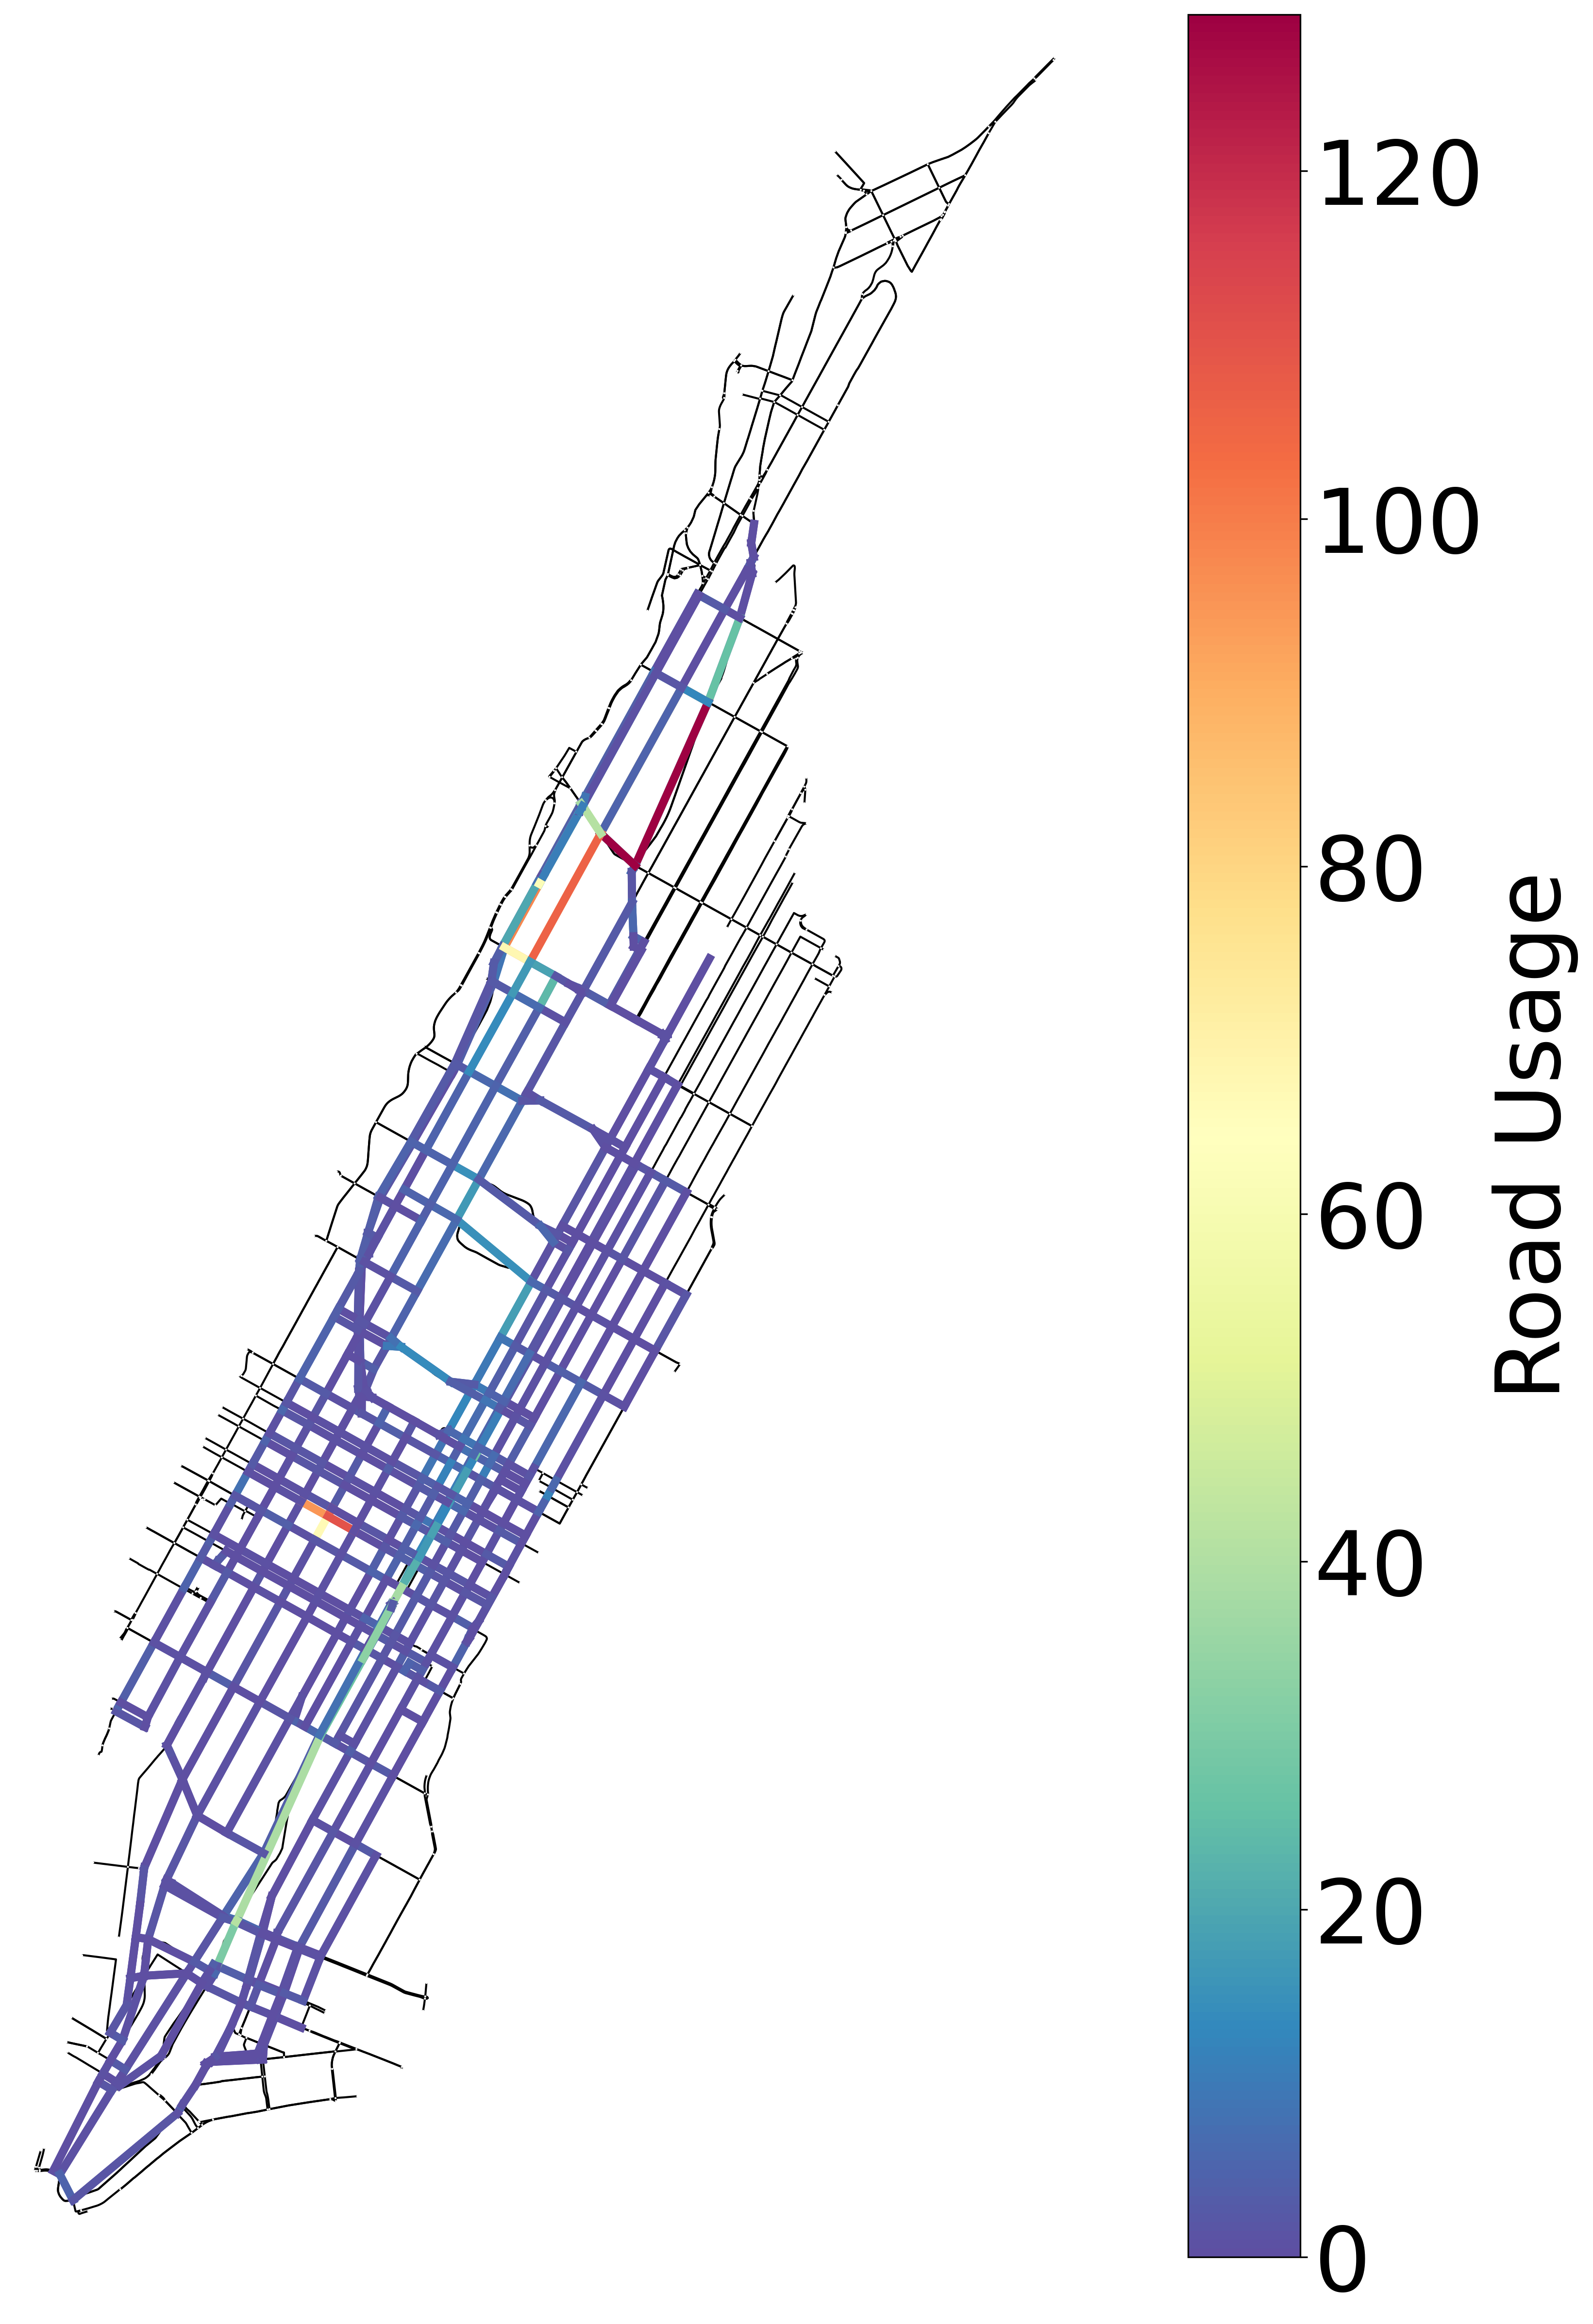
\includegraphics[width=\textwidth]{assets/img/appendix_a/nyc_road_usage_simu4.png}
		\caption{}
		\label{app:fig:nyc_road_usage_simu4}
	\end{subfigure}
	\begin{subfigure}[b]{0.4\textwidth}
		\centering
		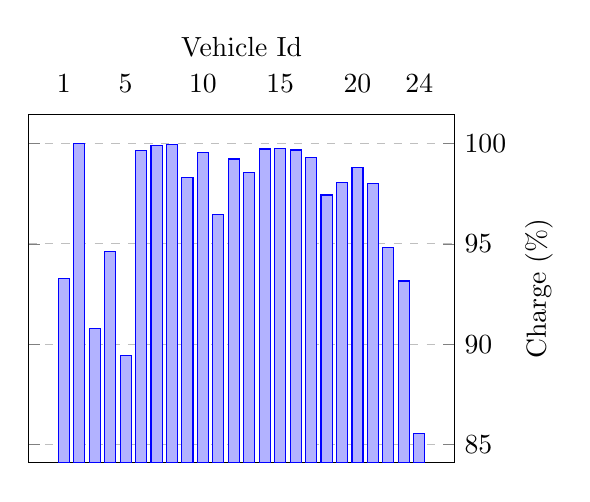
\begin{tikzpicture}
			\begin{axis}[
				ybar,
				xtick=data,
				xtick={1,5, 10,15,20,24},
				xlabel={Vehicle Id},
				ylabel={Charge (\%)},
				bar width=4pt,
				ymajorgrids=true,
				yticklabel pos=right,
				ylabel near ticks,
				grid style=dashed,
				xticklabel pos=right, xlabel near ticks,
				minor x tick num=9,
				xtick style={draw=none},
				width=7cm, 
				height=6cm
				]
				\addplot coordinates{
					(1,93.27138291372177)
					(2,100.0)
					(3,90.78912726438328)
					(4,94.63488886816818)
					(5,89.42500626723746)
					(6,99.66414618819783)
					(7,99.89679061844821)
					(8,99.96727833421122)
					(9,98.30176552168888)
					(10,99.54836646066505)
					(11,96.44722524056257)
					(12,99.23116671701324)
					(13,98.54691633563728)
					(14,99.72911169462172)
					(15,99.73123438245129)
					(16,99.67615569319422)
					(17,99.29704775451592)
					(18,97.43522071175792)
					(19,98.04548532472887)
					(20,98.79371095065098)
					(21,97.99881594873128)
					(22,94.81483442468704)
					(23,93.15136530688466)
					(24,85.55061528376164)
				};			
			\end{axis}
		\end{tikzpicture}
		\caption{ }
		\label{app:fig:charge_vehicle_baseline_cong_simu4}
	\end{subfigure}
	\caption[Overview of System's Performance with Congestion Limits and Less Charging Time]{Overview of System's Performance without Congestion Limits and Less Charging Time.
		\subfigref{app:fig:nyc_road_usage_simu4} illustrates the utilization of the entire road network during the whole shift, while \subfigref{app:fig:charge_vehicle_baseline_cong_simu4} shows averaging charging percentage of the vehicles. 
	}
	\label{app:fig:nyc_analysis_congestions_simu4}
\end{figure}